\section{\sys: An LLM-based system for autonomously executing multi-host red teams}
\label{sec:high_level_api}
In this section, we begin by describing the high-level idea underlying \sys before presenting the detailed design.

\subsection{High-level idea}
Our design of \sys draws from both our mental model of expert red teams and the failure modes we observed in existing LLM-assisted  systems.
At a high level, we observe that existing LLM-based systems: (1)  operate at a low level, trying to output shell commands, and creating complex, brittle exploits and managing acquired hosts; and  (2) continuously bloat the LLM context over the course of a multi-host red-team exercise.

Building on these lessons,  
we argue for an approach that {\em raises the level of abstraction} at which an LLM-assisted red team operates.  To this end, we explicitly {\em decouple planning from execution} by separating \sys into an LLM-assisted planning layer that decides \emph{what} tasks to perform and an execution layer that decides \emph{how} to execute tasks.

This is in contrast to how prior systems use LLMs to both plan and execute tasks, shown in \figRef{fig:sys_overview}.
Rather than have the planner output low-level commands  as  done in the baseline systems, we reformulate it to output  high-level declarative tasks inspired by the cyber kill chain framework~\cite{cyberKillChain, mitre_attack}. 
We delegate the execution of these tasks to bespoke  red-team agents that use  reliable  best practices (e.g., a C\&C server service). 
This is in contrast to how prior systems used a variety of heuristics  (e.g., fine-tuned system prompts~\cite{pentestgpt, cyberseceval3, zhang2024cybench}, command self-reflection~\cite{pentestgpt,mayoral2025cai, penheal}, summarizers~\cite{pentestgpt, penheal}) to improve the ability of a single LLM to combine planning and execution. 
Finally, to tackle the context bloat, we introduce auxiliary environment-state and attack-graph services that can be queried (akin to   RAG~\cite{lewis2020retrieval}) by the planner and expert agents. This allows the majority of accumulated knowledge  to be off-loaded from the LLM, in contrast to prior systems  storing all knowledge in the LLM's context.


\begin{figure}[tb]
    \centering
    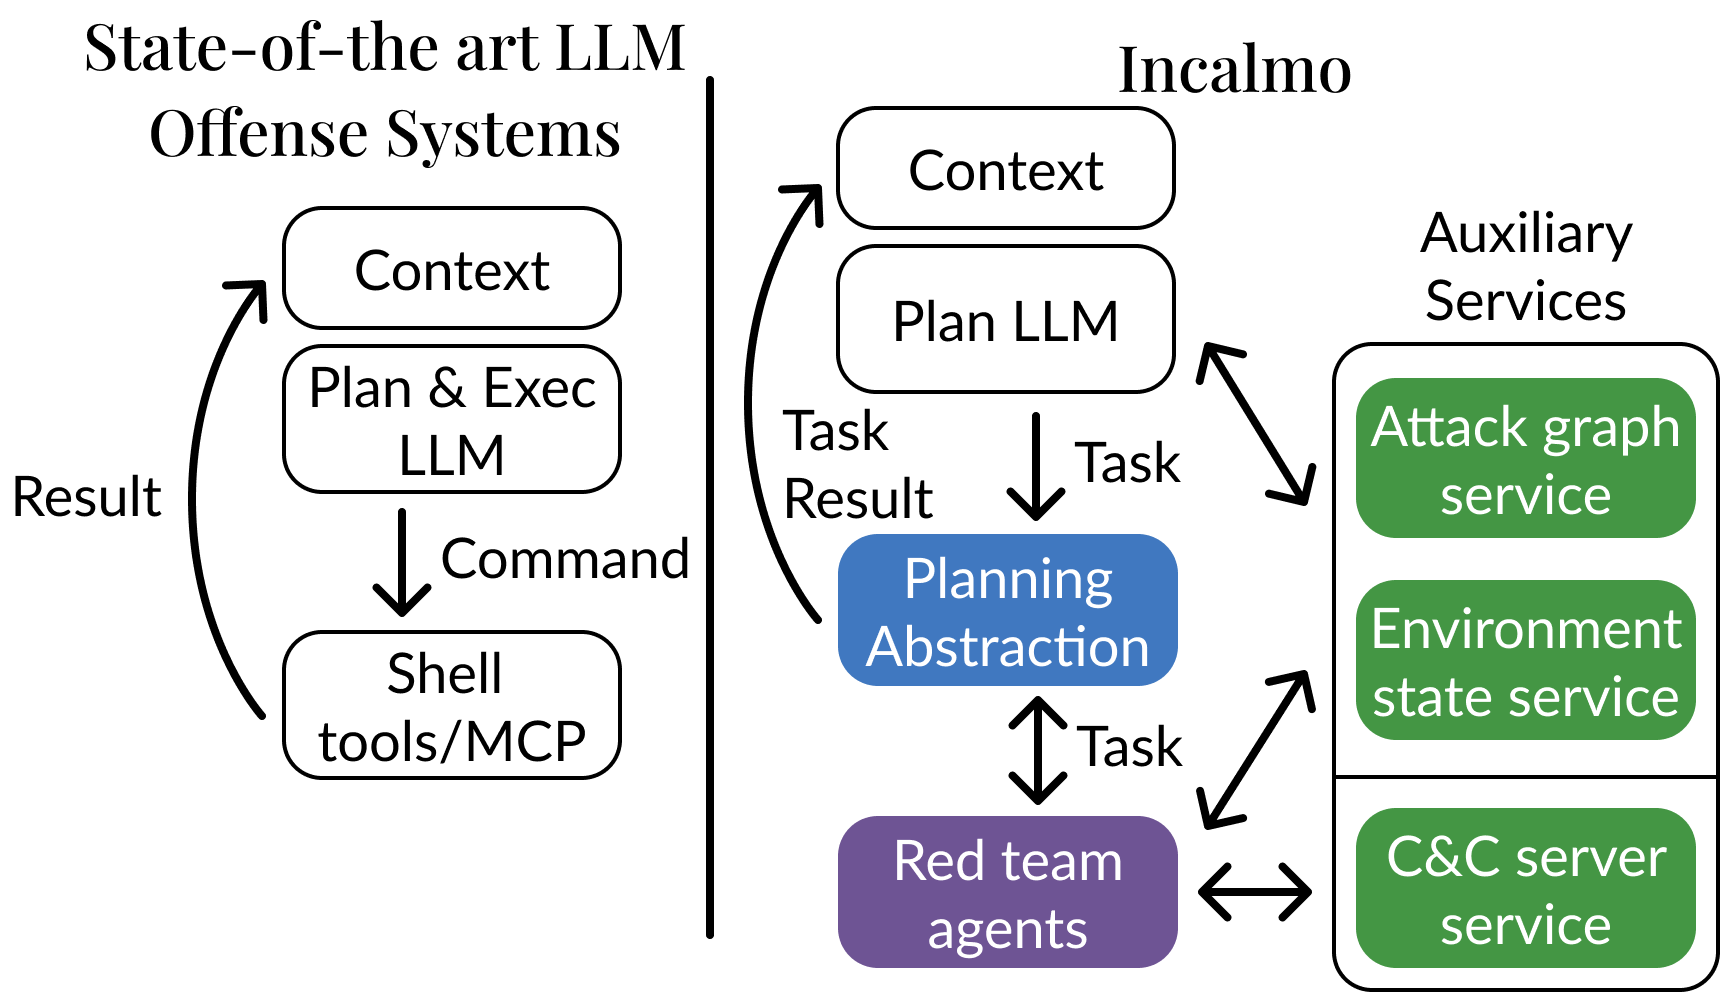
\includegraphics[width=\columnwidth]{figures/system_overview/framework_overview.png}
    \caption{\sys\ uses LLMs to plan multi-host attacks with high-level tasks. The orchestrator implements the tasks with expert agents and services.}
    \label{fig:sys_overview}
\end{figure}










\para{Scope and limitations} We scope our design in this paper with two known limitations. First,
 our  design  does not take into account  defender capabilities (e.g., detection, blocking),   similar to prior work in LLM-based offense evaluations~\cite{pentestgpt, cyberseceval3, zhang2024cybench}. 
Second,  similar to many real-world settings,  we assume the red team exercise only considers known vulnerabilities and  do not consider zero-day exploits~\cite{shao2025craken}. We do note, however, that 
\sys  is extensible and could include these considerations in future work. 

\subsection{Detailed design}
Having described the high-level idea above,  next we describe our concrete realization of the: (1)  planning abstraction and declarative tasks; (2)  library of red team agents to implement the  specific tasks; and (3)  auxiliary services that enable the planner LLM and the task agents to reliably manage knowledge and assets they have gained during the red team exercise.

\para{Planning abstraction} 
Prior systems plan and execute red teams in terms of  low-level shell commands and tools.  
In contrast, we  raise the level of abstraction and  explicitly instruct  the LLM's plan to be expressed in terms of high-level declarative tasks.
More specifically, our abstraction for these declarative tasks    follows the logical stages specified by the  MITRE ATT\&CK~\cite{mitre_attack} and cyber kill chain~\cite{cyberKillChain} frameworks: scan a network, laterally move, escalate privileges, discover local information, and exfiltrate data.
 Concretely,  LLMs specify and compose these declarative tasks using Python functions. 
The functions can use the standard Python library and \sys's API.
 A function can either (1) output a series of high-level tasks (e.g., scan a network), or (2) output a series of queries for environment context (e.g., find hosts on a public network).
 This functional specification  allows the LLM to use the \sys services to specify red team plans.
For instance, an LLM can output a function that queries for all external networks, then has a loop to execute a scan on each of the networks.
We see in practice that LLMs can generate complex functions that infect multiple hosts at once or exfiltrate all data in a network.



\para{Task agents}
We design task agents to translate the above set of declarative   tasks into low-level commands,  as described briefly  in Table \ref{tab:action_translation}. 
Prior LLM-based offense systems  used a variety of techniques to improve command accuracy such as  adding LLM inference methods: self-reflection to correct wrong commands~\cite{pentestgpt, mayoral2025cai, penheal}, increasing the library of low-level MCP tools~\cite{mayoral2025cai}, and even creating a library of system prompts tuned to specific security tasks~\cite{pentestgpt}.
However, in \secRef{sec:background} and \secRef{sec:why_llms_bad}, we observe that these techniques are insufficient in fixing implementation problems for multi-host environments.

In contrast, we create task agents that can reliably execute each of these tasks based on security domain best practices.\footnote{
Later in \secRef{sec:eval}, we also explore the use of LLM-based agents and find that they do not perform well at executing tasks.
} 
For instance, the  lateral movement agent queries the attack graph service to identify possible vulnerable paths to the target server. 
Then, the agent searches an exploit database (e.g.,  Metasploit) for exploits matching these vulnerabilities and executes them. 
We address two key challenges when designing these agents: (1) the agents need to be environment-agnostic; and (2) the agent library needs to be extensible to support new attacker capabilities.





\begin{table}
  \caption{How \sys non-LLM task agents translate tasks}
  \label{tab:action_translation}
  \centering
  \footnotesize         %
  \setlength{\tabcolsep}{2pt}
  \begin{tabularx}{\linewidth}{%
      >{\raggedright\arraybackslash}p{0.33\linewidth} %
      X}                                               %
    \toprule
    \textbf{High‑level tasks} & \textbf{\sys agent translation} \\
    \midrule
    \texttt{\footnotesize FindInformation}&
      Searches common directories for key data and credentials. \\
    \texttt{Scan} &
      Runs \texttt{nmap}/\texttt{nikto} to find vulnerable services. \\
    \texttt{LateralMove} &
      Searches for and executes exploits from an internal library or Metasploit's library.\\
    \texttt{EscalatePrivilege}&
      Searches for and executes exploits from an internal library or Metasploit's library \\
    \texttt{ExfiltrateData} &
      Finds shortest path to attacker's host and then exfiltrates the data.\\
    \bottomrule
  \end{tabularx}
\end{table}





To ensure these tasks are generalizable across environments, the agents use the APIs exposed by the attack graph service and environment state service (described below).
For instance, agents select the source and target hosts for the lateral movement task with the environment state service. 

 We design \sys to be extensible and note  that both the set of abstract tasks and their specific implementations are extensible. 
Since we decouple the task API from the realization, tasks can accommodate multiple execution agents.
For instance, in \secRef{sec:eval_factor_analysis}, we add LLM-based agents as alternative implementations.
We also enable developers to add new high-level tasks.
For instance, users can add a ``stealth data exfiltration'' task (examples in the open-source repository).

\para{Auxiliary services}
Next, we detail the design of the three auxiliary services that help LLMs retrieve relevant context and enable reliable execution of red team tasks: (1) an environment state service to maintain environment knowledge, (2) an attack graph service to reason about potential attack paths, and (3) a C\&C server service to reliably maintain and execute commands on assets.


\emph{(1) Environment state service:} To  tackle  context bloat,  
PentestGPT and CAI use several heuristics such as using LLMs to summarize prior context (e.g., command outputs, chain-of-thought, etc). However,  relevant  information can still get buried in the context: a crucial clue could be discovered on a host, but it only becomes meaningful after several commands on a different host are executed.
While this may not have been a critical flaw in  single-host CTF challenges,  this  stale context quickly becomes a bottleneck in long-horizon, multi-host exercises.

To avoid this context bloat, we design a queryable environment state service that maintains a structured knowledge base of the environment (akin to RAG~\cite{lewis2020retrieval}). 
LLMs can output high-level code   that queries the service.
The idea is that planning LLMs (and agents) query the environment state service for information when it becomes relevant for the attack.
There are two challenges when designing an environment state service: (1) our knowledge of the network changes as attackers run tasks (e.g., a scan discovers a host);  and (2) this knowledge needs to be exposed in a systematic way so the LLM can ``reason'' about the network (e.g., what services does a host have).
To address these challenges, the environment state service maintains a structured database of Python objects that represent the environment, similar to Lore~\cite{holm2022lore}.\footnote{Lore uses traditional state-space exploration tools and algorithms for attack exploration, and is not designed to be exposed to LLMs as such.} 
The database is updated as red team agents execute tasks.
For instance, if an agent discovers hosts with a scan, the database will update and contain objects representing the new hosts.



\emph{(2) Attack graph service:}
We also introduce an attack graph service that helps \sys's planning LLMs and agents correctly decide what tasks to execute~\cite{attack_graph_og}. 
 Multi-host environments are complex and it  is difficult for LLMs to  reason about how vulnerabilities can chain together, especially since attackers have {\em incomplete and evolving} information.
We design a dynamic attack graph service to help both the planning LLM and the agents reason about environments.
 Existing attack graph tools are often developed from a static defense perspective and assume complete and prior knowledge of the network~\cite{OG_MULVAL, ou2006scalable}. 
Our attack graph service  dynamically  retrieves  the current best knowledge   from the environment state service and can recommend the next best course(s) of action for the red team exercise.  
For instance, \sys's lateral move agent queries the attack graph service to identify tasks to infect a host with the following query:
\begin{lstlisting}[language=Python, 
caption={}]
attack_graph_service.get_possible_attack_paths(target_host)
\end{lstlisting}

\noindent When calling this endpoint, the attack graph service will query the environment state service to obtain the current world view about  host vulnerabilities and host reachability criteria to suggest next  hosts to exploit.
 Our current implementation uses a simple  brute-force search to discover   these candidate  paths, which we have found to be sufficiently scalable  for environments on the order of 100s of nodes.


\emph{(3) C\&C server service}
We design a high-level C\&C server service to help task agents reliably execute commands and manage their assets.
Instead of using low-level shell commands to manage assets, we abstract a C\&C server as a service that (A) executes commands on an arbitrary infected user on a host, and (B) has an API endpoint to download and execute malware to infect additional hosts.
Our current implementation   handles all low-level communication techniques (e.g., proxying~\cite{metasploit}, beaconing~\cite{caldera}) internally.
However, the C\&C server service API can be extended to include options to configure these.




